\documentclass[1p]{elsarticle_modified}
%\bibliographystyle{elsarticle-num}

%\usepackage[colorlinks]{hyperref}
%\usepackage{abbrmath_seonhwa} %\Abb, \Ascr, \Acal ,\Abf, \Afrak
\usepackage{amsfonts}
\usepackage{amssymb}
\usepackage{amsmath}
\usepackage{amsthm}
\usepackage{scalefnt}
\usepackage{amsbsy}
\usepackage{kotex}
\usepackage{caption}
\usepackage{subfig}
\usepackage{color}
\usepackage{graphicx}
\usepackage{xcolor} %% white, black, red, green, blue, cyan, magenta, yellow
\usepackage{float}
\usepackage{setspace}
\usepackage{hyperref}

\usepackage{tikz}
\usetikzlibrary{arrows}

\usepackage{multirow}
\usepackage{array} % fixed length table
\usepackage{hhline}

%%%%%%%%%%%%%%%%%%%%%
\makeatletter
\renewcommand*\env@matrix[1][\arraystretch]{%
	\edef\arraystretch{#1}%
	\hskip -\arraycolsep
	\let\@ifnextchar\new@ifnextchar
	\array{*\c@MaxMatrixCols c}}
\makeatother %https://tex.stackexchange.com/questions/14071/how-can-i-increase-the-line-spacing-in-a-matrix
%%%%%%%%%%%%%%%

\usepackage[normalem]{ulem}

\newcommand{\msout}[1]{\ifmmode\text{\sout{\ensuremath{#1}}}\else\sout{#1}\fi}
%SOURCE: \msout is \stkout macro in https://tex.stackexchange.com/questions/20609/strikeout-in-math-mode

\newcommand{\cancel}[1]{
	\ifmmode
	{\color{red}\msout{#1}}
	\else
	{\color{red}\sout{#1}}
	\fi
}

\newcommand{\add}[1]{
	{\color{blue}\uwave{#1}}
}

\newcommand{\replace}[2]{
	\ifmmode
	{\color{red}\msout{#1}}{\color{blue}\uwave{#2}}
	\else
	{\color{red}\sout{#1}}{\color{blue}\uwave{#2}}
	\fi
}

\newcommand{\Sol}{\mathcal{S}} %segment
\newcommand{\D}{D} %diagram
\newcommand{\A}{\mathcal{A}} %arc


%%%%%%%%%%%%%%%%%%%%%%%%%%%%%5 test

\def\sl{\operatorname{\textup{SL}}(2,\Cbb)}
\def\psl{\operatorname{\textup{PSL}}(2,\Cbb)}
\def\quan{\mkern 1mu \triangleright \mkern 1mu}

\theoremstyle{definition}
\newtheorem{thm}{Theorem}[section]
\newtheorem{prop}[thm]{Proposition}
\newtheorem{lem}[thm]{Lemma}
\newtheorem{ques}[thm]{Question}
\newtheorem{cor}[thm]{Corollary}
\newtheorem{defn}[thm]{Definition}
\newtheorem{exam}[thm]{Example}
\newtheorem{rmk}[thm]{Remark}
\newtheorem{alg}[thm]{Algorithm}

\newcommand{\I}{\sqrt{-1}}
\begin{document}

%\begin{frontmatter}
%
%\title{Boundary parabolic representations of knots up to 8 crossings}
%
%%% Group authors per affiliation:
%\author{Yunhi Cho} 
%\address{Department of Mathematics, University of Seoul, Seoul, Korea}
%\ead{yhcho@uos.ac.kr}
%
%
%\author{Seonhwa Kim} %\fnref{s_kim}}
%\address{Center for Geometry and Physics, Institute for Basic Science, Pohang, 37673, Korea}
%\ead{ryeona17@ibs.re.kr}
%
%\author{Hyuk Kim}
%\address{Department of Mathematical Sciences, Seoul National University, Seoul 08826, Korea}
%\ead{hyukkim@snu.ac.kr}
%
%\author{Seokbeom Yoon}
%\address{Department of Mathematical Sciences, Seoul National University, Seoul, 08826,  Korea}
%\ead{sbyoon15@snu.ac.kr}
%
%\begin{abstract}
%We find all boundary parabolic representation of knots up to 8 crossings.
%
%\end{abstract}
%\begin{keyword}
%    \MSC[2010] 57M25 
%\end{keyword}
%
%\end{frontmatter}

%\linenumbers
%\tableofcontents
%
\newcommand\colored[1]{\textcolor{white}{\rule[-0.35ex]{0.8em}{1.4ex}}\kern-0.8em\color{red} #1}%
%\newcommand\colored[1]{\textcolor{white}{ #1}\kern-2.17ex	\textcolor{white}{ #1}\kern-1.81ex	\textcolor{white}{ #1}\kern-2.15ex\color{red}#1	}

{\Large $\underline{12n_{0653}~(K12n_{0653})}$}

\setlength{\tabcolsep}{10pt}
\renewcommand{\arraystretch}{1.6}
\vspace{1cm}\begin{tabular}{m{100pt}>{\centering\arraybackslash}m{274pt}}
\multirow{5}{120pt}{
	\centering
	\includegraphics[width=112pt]{../../../GIT/diagram.site/Diagrams/png/2742_12n_0653.png}\\
\ \ \ A knot diagram\footnotemark}&
\allowdisplaybreaks
\textbf{Linearized knot diagam} \\
\cline{2-2}
 &
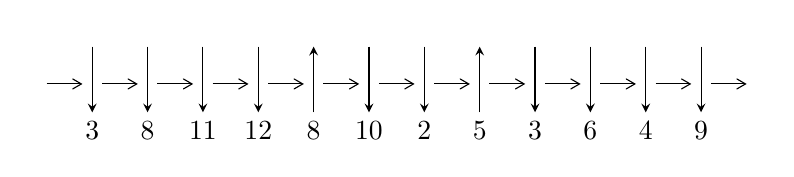
\begin{tikzpicture}[x=20pt, y=17pt]
	% nodes
	\node (C0) at (0, 0) {};
	\node (C1) at (1, 0) {};
	\node (C1U) at (1, +1) {};
	\node (C1D) at (1, -1) {3};

	\node (C2) at (2, 0) {};
	\node (C2U) at (2, +1) {};
	\node (C2D) at (2, -1) {8};

	\node (C3) at (3, 0) {};
	\node (C3U) at (3, +1) {};
	\node (C3D) at (3, -1) {11};

	\node (C4) at (4, 0) {};
	\node (C4U) at (4, +1) {};
	\node (C4D) at (4, -1) {12};

	\node (C5) at (5, 0) {};
	\node (C5U) at (5, +1) {};
	\node (C5D) at (5, -1) {8};

	\node (C6) at (6, 0) {};
	\node (C6U) at (6, +1) {};
	\node (C6D) at (6, -1) {10};

	\node (C7) at (7, 0) {};
	\node (C7U) at (7, +1) {};
	\node (C7D) at (7, -1) {2};

	\node (C8) at (8, 0) {};
	\node (C8U) at (8, +1) {};
	\node (C8D) at (8, -1) {5};

	\node (C9) at (9, 0) {};
	\node (C9U) at (9, +1) {};
	\node (C9D) at (9, -1) {3};

	\node (C10) at (10, 0) {};
	\node (C10U) at (10, +1) {};
	\node (C10D) at (10, -1) {6};

	\node (C11) at (11, 0) {};
	\node (C11U) at (11, +1) {};
	\node (C11D) at (11, -1) {4};

	\node (C12) at (12, 0) {};
	\node (C12U) at (12, +1) {};
	\node (C12D) at (12, -1) {9};
	\node (C13) at (13, 0) {};

	% arrows
	\draw[->,>={angle 60}]
	(C0) edge (C1) (C1) edge (C2) (C2) edge (C3) (C3) edge (C4) (C4) edge (C5) (C5) edge (C6) (C6) edge (C7) (C7) edge (C8) (C8) edge (C9) (C9) edge (C10) (C10) edge (C11) (C11) edge (C12) (C12) edge (C13) ;	\draw[->,>=stealth]
	(C1U) edge (C1D) (C2U) edge (C2D) (C3U) edge (C3D) (C4U) edge (C4D) (C5D) edge (C5U) (C6U) edge (C6D) (C7U) edge (C7D) (C8D) edge (C8U) (C9U) edge (C9D) (C10U) edge (C10D) (C11U) edge (C11D) (C12U) edge (C12D) ;
	\end{tikzpicture} \\
\hhline{~~} \\& 
\textbf{Solving Sequence} \\ \cline{2-2} 
 &
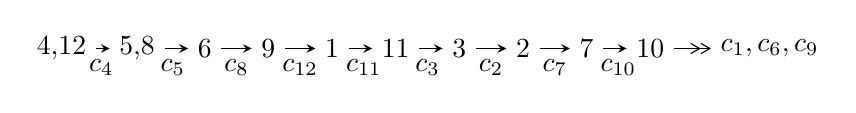
\begin{tikzpicture}[x=23pt, y=7pt]
	% node
	\node (A0) at (-1/8, 0) {4,12};
	\node (A1) at (17/16, 0) {5,8};
	\node (A2) at (17/8, 0) {6};
	\node (A3) at (25/8, 0) {9};
	\node (A4) at (33/8, 0) {1};
	\node (A5) at (41/8, 0) {11};
	\node (A6) at (49/8, 0) {3};
	\node (A7) at (57/8, 0) {2};
	\node (A8) at (65/8, 0) {7};
	\node (A9) at (73/8, 0) {10};
	\node (C1) at (1/2, -1) {$c_{4}$};
	\node (C2) at (13/8, -1) {$c_{5}$};
	\node (C3) at (21/8, -1) {$c_{8}$};
	\node (C4) at (29/8, -1) {$c_{12}$};
	\node (C5) at (37/8, -1) {$c_{11}$};
	\node (C6) at (45/8, -1) {$c_{3}$};
	\node (C7) at (53/8, -1) {$c_{2}$};
	\node (C8) at (61/8, -1) {$c_{7}$};
	\node (C9) at (69/8, -1) {$c_{10}$};
	\node (A10) at (11, 0) {$c_{1},c_{6},c_{9}$};

	% edge
	\draw[->,>=stealth]	
	(A0) edge (A1) (A1) edge (A2) (A2) edge (A3) (A3) edge (A4) (A4) edge (A5) (A5) edge (A6) (A6) edge (A7) (A7) edge (A8) (A8) edge (A9) ;
	\draw[->>,>={angle 60}]	
	(A9) edge (A10);
\end{tikzpicture} \\ 

\end{tabular} \\

\footnotetext{
The image of knot diagram is generated by the software ``\textbf{Draw programme}" developed by Andrew Bartholomew(\url{http://www.layer8.co.uk/maths/draw/index.htm\#Running-draw}), where we modified some parts for our purpose(\url{https://github.com/CATsTAILs/LinksPainter}).
}\phantom \\ \newline 
\centering \textbf{Ideals for irreducible components\footnotemark of $X_{\text{par}}$} 
 
\begin{align*}
I^u_{1}&=\langle 
15 u^{19}+52 u^{18}+\cdots+b-21,\;21 u^{19}+75 u^{18}+\cdots+2 a-23,\;u^{20}+5 u^{19}+\cdots+u-2\rangle \\
I^u_{2}&=\langle 
2 u^{12}-2 u^{11}-11 u^{10}+8 u^9+23 u^8-5 u^7-22 u^6-13 u^5+4 u^4+16 u^3+8 u^2+b- u-2,\\
\phantom{I^u_{2}}&\phantom{= \langle  }2 u^{12}-2 u^{11}-12 u^{10}+9 u^9+28 u^8-9 u^7-31 u^6-10 u^5+11 u^4+20 u^3+8 u^2+a-6 u-5,\\
\phantom{I^u_{2}}&\phantom{= \langle  }u^{13}-2 u^{12}-5 u^{11}+10 u^{10}+10 u^9-16 u^8-13 u^7+6 u^6+12 u^5+8 u^4-4 u^3-7 u^2-2 u+1\rangle \\
I^u_{3}&=\langle 
u^5- u^4-2 u^3- a u+u^2+b+u+1,\;- u^5 a-4 u^5+4 u^3 a+u^4+11 u^3+a^2-3 a u+u^2-2 a-4 u-6,\\
\phantom{I^u_{3}}&\phantom{= \langle  }u^6- u^5-3 u^4+2 u^3+2 u^2+u-1\rangle \\
\\
\end{align*}
\raggedright * 3 irreducible components of $\dim_{\mathbb{C}}=0$, with total 45 representations.\\
\footnotetext{All coefficients of polynomials are rational numbers. But the coefficients are sometimes approximated in decimal forms when there is not enough margin.}
\newpage
\renewcommand{\arraystretch}{1}
\centering \section*{I. $I^u_{1}= \langle 15 u^{19}+52 u^{18}+\cdots+b-21,\;21 u^{19}+75 u^{18}+\cdots+2 a-23,\;u^{20}+5 u^{19}+\cdots+u-2 \rangle$}
\flushleft \textbf{(i) Arc colorings}\\
\begin{tabular}{m{7pt} m{180pt} m{7pt} m{180pt} }
\flushright $a_{4}=$&$\begin{pmatrix}1\\0\end{pmatrix}$ \\
\flushright $a_{12}=$&$\begin{pmatrix}0\\u\end{pmatrix}$ \\
\flushright $a_{5}=$&$\begin{pmatrix}1\\u^2\end{pmatrix}$ \\
\flushright $a_{8}=$&$\begin{pmatrix}-10.5000 u^{19}-37.5000 u^{18}+\cdots-17.5000 u+11.5000\\-15 u^{19}-52 u^{18}+\cdots-22 u+21\end{pmatrix}$ \\
\flushright $a_{6}=$&$\begin{pmatrix}\frac{11}{2} u^{19}+\frac{37}{2} u^{18}+\cdots+\frac{11}{2} u-\frac{11}{2}\\9 u^{19}+30 u^{18}+\cdots+12 u-11\end{pmatrix}$ \\
\flushright $a_{9}=$&$\begin{pmatrix}-\frac{5}{2} u^{19}-\frac{19}{2} u^{18}+\cdots-\frac{7}{2} u+\frac{5}{2}\\4 u^{19}+13 u^{18}+\cdots+6 u-3\end{pmatrix}$ \\
\flushright $a_{1}=$&$\begin{pmatrix}-\frac{5}{2} u^{19}-\frac{17}{2} u^{18}+\cdots-\frac{7}{2} u+\frac{7}{2}\\-6 u^{19}-20 u^{18}+\cdots-7 u+7\end{pmatrix}$ \\
\flushright $a_{11}=$&$\begin{pmatrix}u\\u\end{pmatrix}$ \\
\flushright $a_{3}=$&$\begin{pmatrix}- u^2+1\\- u^2\end{pmatrix}$ \\
\flushright $a_{2}=$&$\begin{pmatrix}\frac{5}{2} u^{19}+\frac{19}{2} u^{18}+\cdots+\frac{9}{2} u-\frac{7}{2}\\3 u^{19}+12 u^{18}+\cdots+7 u-5\end{pmatrix}$ \\
\flushright $a_{7}=$&$\begin{pmatrix}-23 u^{19}-80 u^{18}+\cdots-34 u+27\\-32 u^{19}-110 u^{18}+\cdots-45 u+42\end{pmatrix}$ \\
\flushright $a_{10}=$&$\begin{pmatrix}-22.5000 u^{19}-78.5000 u^{18}+\cdots-33.5000 u+27.5000\\-29 u^{19}-100 u^{18}+\cdots-41 u+39\end{pmatrix}$\\&\end{tabular}
\flushleft \textbf{(ii) Obstruction class $= -1$}\\~\\
\flushleft \textbf{(iii) Cusp Shapes $= -15 u^{19}-52 u^{18}+51 u^{17}+300 u^{16}-63 u^{15}-689 u^{14}+302 u^{13}+905 u^{12}-1067 u^{11}-777 u^{10}+1394 u^9+39 u^8-722 u^7+587 u^6+181 u^5+7 u^4+174 u^3-147 u^2-9 u+12$}\\~\\
\newpage\renewcommand{\arraystretch}{1}
\flushleft \textbf{(iv) u-Polynomials at the component}\newline \\
\begin{tabular}{m{50pt}|m{274pt}}
Crossings & \hspace{64pt}u-Polynomials at each crossing \\
\hline $$\begin{aligned}c_{1}\end{aligned}$$&$\begin{aligned}
&u^{20}+31 u^{19}+\cdots-5 u+1
\end{aligned}$\\
\hline $$\begin{aligned}c_{2},c_{7},c_{12}\end{aligned}$$&$\begin{aligned}
&u^{20}+u^{19}+\cdots-3 u-1
\end{aligned}$\\
\hline $$\begin{aligned}c_{3},c_{4},c_{11}\end{aligned}$$&$\begin{aligned}
&u^{20}+5 u^{19}+\cdots+u-2
\end{aligned}$\\
\hline $$\begin{aligned}c_{5},c_{8}\end{aligned}$$&$\begin{aligned}
&u^{20}- u^{19}+\cdots-7 u+1
\end{aligned}$\\
\hline $$\begin{aligned}c_{6},c_{10}\end{aligned}$$&$\begin{aligned}
&u^{20}+14 u^{19}+\cdots+608 u+64
\end{aligned}$\\
\hline $$\begin{aligned}c_{9}\end{aligned}$$&$\begin{aligned}
&u^{20}-26 u^{18}+\cdots-494 u-599
\end{aligned}$\\
\hline
\end{tabular}\\~\\
\newpage\renewcommand{\arraystretch}{1}
\flushleft \textbf{(v) Riley Polynomials at the component}\newline \\
\begin{tabular}{m{50pt}|m{274pt}}
Crossings & \hspace{64pt}Riley Polynomials at each crossing \\
\hline $$\begin{aligned}c_{1}\end{aligned}$$&$\begin{aligned}
&y^{20}-103 y^{19}+\cdots-159 y+1
\end{aligned}$\\
\hline $$\begin{aligned}c_{2},c_{7},c_{12}\end{aligned}$$&$\begin{aligned}
&y^{20}-31 y^{19}+\cdots+5 y+1
\end{aligned}$\\
\hline $$\begin{aligned}c_{3},c_{4},c_{11}\end{aligned}$$&$\begin{aligned}
&y^{20}-21 y^{19}+\cdots-61 y+4
\end{aligned}$\\
\hline $$\begin{aligned}c_{5},c_{8}\end{aligned}$$&$\begin{aligned}
&y^{20}+29 y^{19}+\cdots-55 y+1
\end{aligned}$\\
\hline $$\begin{aligned}c_{6},c_{10}\end{aligned}$$&$\begin{aligned}
&y^{20}+6 y^{19}+\cdots-33792 y+4096
\end{aligned}$\\
\hline $$\begin{aligned}c_{9}\end{aligned}$$&$\begin{aligned}
&y^{20}-52 y^{19}+\cdots+2577254 y+358801
\end{aligned}$\\
\hline
\end{tabular}\\~\\
\newpage\flushleft \textbf{(vi) Complex Volumes and Cusp Shapes}
$$\begin{array}{c|c|c}  
\text{Solutions to }I^u_{1}& \I (\text{vol} + \sqrt{-1}CS) & \text{Cusp shape}\\
 \hline 
\begin{aligned}
u &= \phantom{-}0.537648 + 0.858586 I \\
a &= \phantom{-}0.960669 - 0.049342 I \\
b &= -0.558866 - 0.798289 I\end{aligned}
 & -14.2098 + 2.1239 I & -11.72729 + 0.16245 I \\ \hline\begin{aligned}
u &= \phantom{-}0.537648 - 0.858586 I \\
a &= \phantom{-}0.960669 + 0.049342 I \\
b &= -0.558866 + 0.798289 I\end{aligned}
 & -14.2098 - 2.1239 I & -11.72729 - 0.16245 I \\ \hline\begin{aligned}
u &= \phantom{-}0.606622 + 0.819368 I \\
a &= -0.914544 - 0.419396 I \\
b &= \phantom{-}0.211143 + 1.003760 I\end{aligned}
 & -14.4361 - 7.6779 I & -11.74067 + 4.57873 I \\ \hline\begin{aligned}
u &= \phantom{-}0.606622 - 0.819368 I \\
a &= -0.914544 + 0.419396 I \\
b &= \phantom{-}0.211143 - 1.003760 I\end{aligned}
 & -14.4361 + 7.6779 I & -11.74067 - 4.57873 I \\ \hline\begin{aligned}
u &= -1.223290 + 0.229738 I \\
a &= -0.518734 - 0.448442 I \\
b &= -0.737585 - 0.429401 I\end{aligned}
 & -1.41396 + 1.68379 I & -7.75011 + 2.58763 I \\ \hline\begin{aligned}
u &= -1.223290 - 0.229738 I \\
a &= -0.518734 + 0.448442 I \\
b &= -0.737585 + 0.429401 I\end{aligned}
 & -1.41396 - 1.68379 I & -7.75011 - 2.58763 I \\ \hline\begin{aligned}
u &= -0.087774 + 0.628145 I \\
a &= \phantom{-}0.205193 + 0.654515 I \\
b &= \phantom{-}0.429141 - 0.071442 I\end{aligned}
 & \phantom{-}2.02337 + 1.45900 I & -2.57228 - 5.20755 I \\ \hline\begin{aligned}
u &= -0.087774 - 0.628145 I \\
a &= \phantom{-}0.205193 - 0.654515 I \\
b &= \phantom{-}0.429141 + 0.071442 I\end{aligned}
 & \phantom{-}2.02337 - 1.45900 I & -2.57228 + 5.20755 I \\ \hline\begin{aligned}
u &= \phantom{-}1.382330 + 0.213207 I \\
a &= -0.232569 + 0.103641 I \\
b &= \phantom{-}0.343585 - 0.093682 I\end{aligned}
 & -2.65671 - 4.43053 I & -10.17327 + 4.41788 I \\ \hline\begin{aligned}
u &= \phantom{-}1.382330 - 0.213207 I \\
a &= -0.232569 - 0.103641 I \\
b &= \phantom{-}0.343585 + 0.093682 I\end{aligned}
 & -2.65671 + 4.43053 I & -10.17327 - 4.41788 I\\
 \hline 
 \end{array}$$\newpage$$\begin{array}{c|c|c}  
\text{Solutions to }I^u_{1}& \I (\text{vol} + \sqrt{-1}CS) & \text{Cusp shape}\\
 \hline 
\begin{aligned}
u &= \phantom{-}1.43646\phantom{ +0.000000I} \\
a &= \phantom{-}0.235964\phantom{ +0.000000I} \\
b &= -0.338953\phantom{ +0.000000I}\end{aligned}
 & -6.53090\phantom{ +0.000000I} & -14.6160\phantom{ +0.000000I} \\ \hline\begin{aligned}
u &= -1.51134 + 0.02336 I \\
a &= -0.24536 - 2.15134 I \\
b &= -0.42108 - 3.24569 I\end{aligned}
 & -7.13768 + 2.65728 I & -12.42433 - 2.06390 I \\ \hline\begin{aligned}
u &= -1.51134 - 0.02336 I \\
a &= -0.24536 + 2.15134 I \\
b &= -0.42108 + 3.24569 I\end{aligned}
 & -7.13768 - 2.65728 I & -12.42433 + 2.06390 I \\ \hline\begin{aligned}
u &= \phantom{-}0.418033 + 0.095358 I \\
a &= -0.16881 + 1.84075 I \\
b &= \phantom{-}0.246100 - 0.753394 I\end{aligned}
 & -0.61706 - 2.23609 I & -3.44792 + 0.63650 I \\ \hline\begin{aligned}
u &= \phantom{-}0.418033 - 0.095358 I \\
a &= -0.16881 - 1.84075 I \\
b &= \phantom{-}0.246100 + 0.753394 I\end{aligned}
 & -0.61706 + 2.23609 I & -3.44792 - 0.63650 I \\ \hline\begin{aligned}
u &= -1.56523 + 0.31596 I \\
a &= \phantom{-}0.97491 - 1.39039 I \\
b &= \phantom{-}1.08666 - 2.48431 I\end{aligned}
 & \phantom{-}18.4230 + 2.2284 I & -14.3978 - 0.8992 I \\ \hline\begin{aligned}
u &= -1.56523 - 0.31596 I \\
a &= \phantom{-}0.97491 + 1.39039 I \\
b &= \phantom{-}1.08666 + 2.48431 I\end{aligned}
 & \phantom{-}18.4230 - 2.2284 I & -14.3978 + 0.8992 I \\ \hline\begin{aligned}
u &= -1.58137 + 0.27874 I \\
a &= -0.51960 + 1.97559 I \\
b &= -0.27100 + 3.26896 I\end{aligned}
 & \phantom{-}17.8528 + 11.7492 I & -14.2038 - 4.7569 I \\ \hline\begin{aligned}
u &= -1.58137 - 0.27874 I \\
a &= -0.51960 - 1.97559 I \\
b &= -0.27100 - 3.26896 I\end{aligned}
 & \phantom{-}17.8528 - 11.7492 I & -14.2038 + 4.7569 I \\ \hline\begin{aligned}
u &= -0.387724\phantom{ +0.000000I} \\
a &= -0.818265\phantom{ +0.000000I} \\
b &= -0.317261\phantom{ +0.000000I}\end{aligned}
 & -0.639359\phantom{ +0.000000I} & -15.5090\phantom{ +0.000000I}\\
 \hline 
 \end{array}$$\newpage\newpage\renewcommand{\arraystretch}{1}
\centering \section*{II. $I^u_{2}= \langle 2 u^{12}-2 u^{11}+\cdots+b-2,\;2 u^{12}-2 u^{11}+\cdots+a-5,\;u^{13}-2 u^{12}+\cdots-2 u+1 \rangle$}
\flushleft \textbf{(i) Arc colorings}\\
\begin{tabular}{m{7pt} m{180pt} m{7pt} m{180pt} }
\flushright $a_{4}=$&$\begin{pmatrix}1\\0\end{pmatrix}$ \\
\flushright $a_{12}=$&$\begin{pmatrix}0\\u\end{pmatrix}$ \\
\flushright $a_{5}=$&$\begin{pmatrix}1\\u^2\end{pmatrix}$ \\
\flushright $a_{8}=$&$\begin{pmatrix}-2 u^{12}+2 u^{11}+\cdots+6 u+5\\-2 u^{12}+2 u^{11}+\cdots+u+2\end{pmatrix}$ \\
\flushright $a_{6}=$&$\begin{pmatrix}3 u^{12}-3 u^{11}+\cdots-5 u-5\\3 u^{12}-2 u^{11}+\cdots+17 u^2-3\end{pmatrix}$ \\
\flushright $a_{9}=$&$\begin{pmatrix}-2 u^{12}+3 u^{11}+\cdots+9 u+5\\- u^{12}+2 u^{11}+\cdots+3 u+1\end{pmatrix}$ \\
\flushright $a_{1}=$&$\begin{pmatrix}u^{12}-3 u^{11}+\cdots-17 u-7\\- u^{11}+u^{10}+5 u^9-3 u^8-10 u^7+9 u^5+7 u^4-6 u^2-4 u-1\end{pmatrix}$ \\
\flushright $a_{11}=$&$\begin{pmatrix}u\\u\end{pmatrix}$ \\
\flushright $a_{3}=$&$\begin{pmatrix}- u^2+1\\- u^2\end{pmatrix}$ \\
\flushright $a_{2}=$&$\begin{pmatrix}- u^{12}- u^{11}+\cdots-15 u-4\\-3 u^{12}+u^{11}+\cdots-7 u+1\end{pmatrix}$ \\
\flushright $a_{7}=$&$\begin{pmatrix}5 u^{12}-6 u^{11}+\cdots-10 u-9\\5 u^{12}-4 u^{11}+\cdots+u-6\end{pmatrix}$ \\
\flushright $a_{10}=$&$\begin{pmatrix}-3 u^{12}+3 u^{11}+\cdots+5 u+5\\-4 u^{12}+4 u^{11}+\cdots+u+3\end{pmatrix}$\\&\end{tabular}
\flushleft \textbf{(ii) Obstruction class $= 1$}\\~\\
\flushleft \textbf{(iii) Cusp Shapes $= -4 u^{12}+9 u^{11}+17 u^{10}-41 u^9-27 u^8+56 u^7+32 u^6-11 u^5-30 u^4-29 u^3+8 u^2+12 u-8$}\\~\\
\newpage\renewcommand{\arraystretch}{1}
\flushleft \textbf{(iv) u-Polynomials at the component}\newline \\
\begin{tabular}{m{50pt}|m{274pt}}
Crossings & \hspace{64pt}u-Polynomials at each crossing \\
\hline $$\begin{aligned}c_{1}\end{aligned}$$&$\begin{aligned}
&u^{13}-15 u^{12}+\cdots+9 u-1
\end{aligned}$\\
\hline $$\begin{aligned}c_{2}\end{aligned}$$&$\begin{aligned}
&u^{13}+u^{12}+\cdots+3 u-1
\end{aligned}$\\
\hline $$\begin{aligned}c_{3},c_{4}\end{aligned}$$&$\begin{aligned}
&u^{13}-2 u^{12}+\cdots-2 u+1
\end{aligned}$\\
\hline $$\begin{aligned}c_{5}\end{aligned}$$&$\begin{aligned}
&u^{13}- u^{12}+\cdots+u-1
\end{aligned}$\\
\hline $$\begin{aligned}c_{6}\end{aligned}$$&$\begin{aligned}
&u^{13}+u^{12}+\cdots+u+1
\end{aligned}$\\
\hline $$\begin{aligned}c_{7},c_{12}\end{aligned}$$&$\begin{aligned}
&u^{13}- u^{12}+\cdots+3 u+1
\end{aligned}$\\
\hline $$\begin{aligned}c_{8}\end{aligned}$$&$\begin{aligned}
&u^{13}+u^{12}+\cdots+u+1
\end{aligned}$\\
\hline $$\begin{aligned}c_{9}\end{aligned}$$&$\begin{aligned}
&u^{13}-6 u^{11}-8 u^{10}+7 u^8+3 u^7+16 u^6-2 u^5+14 u^4-3 u^3+6 u^2+1
\end{aligned}$\\
\hline $$\begin{aligned}c_{10}\end{aligned}$$&$\begin{aligned}
&u^{13}- u^{12}+\cdots+u-1
\end{aligned}$\\
\hline $$\begin{aligned}c_{11}\end{aligned}$$&$\begin{aligned}
&u^{13}+2 u^{12}+\cdots-2 u-1
\end{aligned}$\\
\hline
\end{tabular}\\~\\
\newpage\renewcommand{\arraystretch}{1}
\flushleft \textbf{(v) Riley Polynomials at the component}\newline \\
\begin{tabular}{m{50pt}|m{274pt}}
Crossings & \hspace{64pt}Riley Polynomials at each crossing \\
\hline $$\begin{aligned}c_{1}\end{aligned}$$&$\begin{aligned}
&y^{13}-31 y^{12}+\cdots-15 y-1
\end{aligned}$\\
\hline $$\begin{aligned}c_{2},c_{7},c_{12}\end{aligned}$$&$\begin{aligned}
&y^{13}-15 y^{12}+\cdots+9 y-1
\end{aligned}$\\
\hline $$\begin{aligned}c_{3},c_{4},c_{11}\end{aligned}$$&$\begin{aligned}
&y^{13}-14 y^{12}+\cdots+18 y-1
\end{aligned}$\\
\hline $$\begin{aligned}c_{5},c_{8}\end{aligned}$$&$\begin{aligned}
&y^{13}+5 y^{12}+\cdots-7 y-1
\end{aligned}$\\
\hline $$\begin{aligned}c_{6},c_{10}\end{aligned}$$&$\begin{aligned}
&y^{13}+7 y^{12}+\cdots-5 y-1
\end{aligned}$\\
\hline $$\begin{aligned}c_{9}\end{aligned}$$&$\begin{aligned}
&y^{13}-12 y^{12}+\cdots-12 y-1
\end{aligned}$\\
\hline
\end{tabular}\\~\\
\newpage\flushleft \textbf{(vi) Complex Volumes and Cusp Shapes}
$$\begin{array}{c|c|c}  
\text{Solutions to }I^u_{2}& \I (\text{vol} + \sqrt{-1}CS) & \text{Cusp shape}\\
 \hline 
\begin{aligned}
u &= -1.132140 + 0.168986 I \\
a &= \phantom{-}0.092976 + 0.325055 I \\
b &= -0.160192 - 0.352296 I\end{aligned}
 & -1.75574 + 2.59120 I & -12.09350 - 3.87877 I \\ \hline\begin{aligned}
u &= -1.132140 - 0.168986 I \\
a &= \phantom{-}0.092976 - 0.325055 I \\
b &= -0.160192 + 0.352296 I\end{aligned}
 & -1.75574 - 2.59120 I & -12.09350 + 3.87877 I \\ \hline\begin{aligned}
u &= -0.189605 + 0.771385 I \\
a &= \phantom{-}0.646314 + 0.286377 I \\
b &= -0.343451 + 0.444258 I\end{aligned}
 & \phantom{-}0.707606 + 0.983665 I & -10.21762 - 1.58969 I \\ \hline\begin{aligned}
u &= -0.189605 - 0.771385 I \\
a &= \phantom{-}0.646314 - 0.286377 I \\
b &= -0.343451 - 0.444258 I\end{aligned}
 & \phantom{-}0.707606 - 0.983665 I & -10.21762 + 1.58969 I \\ \hline\begin{aligned}
u &= \phantom{-}1.27456\phantom{ +0.000000I} \\
a &= -2.12141\phantom{ +0.000000I} \\
b &= -2.70385\phantom{ +0.000000I}\end{aligned}
 & -10.1403\phantom{ +0.000000I} & -16.1260\phantom{ +0.000000I} \\ \hline\begin{aligned}
u &= -0.596279 + 0.393194 I \\
a &= -0.433017 + 0.867082 I \\
b &= -0.082733 - 0.687283 I\end{aligned}
 & -1.18520 + 2.76688 I & -11.52015 - 6.83060 I \\ \hline\begin{aligned}
u &= -0.596279 - 0.393194 I \\
a &= -0.433017 - 0.867082 I \\
b &= -0.082733 + 0.687283 I\end{aligned}
 & -1.18520 - 2.76688 I & -11.52015 + 6.83060 I \\ \hline\begin{aligned}
u &= \phantom{-}1.369650 + 0.339979 I \\
a &= \phantom{-}0.746659 + 0.696939 I \\
b &= \phantom{-}0.78571 + 1.20841 I\end{aligned}
 & -4.20868 - 5.03112 I & -13.5740 + 4.7480 I \\ \hline\begin{aligned}
u &= \phantom{-}1.369650 - 0.339979 I \\
a &= \phantom{-}0.746659 - 0.696939 I \\
b &= \phantom{-}0.78571 - 1.20841 I\end{aligned}
 & -4.20868 + 5.03112 I & -13.5740 - 4.7480 I \\ \hline\begin{aligned}
u &= -1.51524\phantom{ +0.000000I} \\
a &= -0.421908\phantom{ +0.000000I} \\
b &= \phantom{-}0.639294\phantom{ +0.000000I}\end{aligned}
 & -12.9834\phantom{ +0.000000I} & -12.2240\phantom{ +0.000000I}\\
 \hline 
 \end{array}$$\newpage$$\begin{array}{c|c|c}  
\text{Solutions to }I^u_{2}& \I (\text{vol} + \sqrt{-1}CS) & \text{Cusp shape}\\
 \hline 
\begin{aligned}
u &= \phantom{-}1.53980 + 0.14093 I \\
a &= -0.10346 - 1.87763 I \\
b &= \phantom{-}0.10530 - 2.90577 I\end{aligned}
 & -8.24712 - 4.85635 I & -12.41808 + 4.09970 I \\ \hline\begin{aligned}
u &= \phantom{-}1.53980 - 0.14093 I \\
a &= -0.10346 + 1.87763 I \\
b &= \phantom{-}0.10530 + 2.90577 I\end{aligned}
 & -8.24712 + 4.85635 I & -12.41808 - 4.09970 I \\ \hline\begin{aligned}
u &= \phantom{-}0.257830\phantom{ +0.000000I} \\
a &= \phantom{-}5.64437\phantom{ +0.000000I} \\
b &= \phantom{-}1.45529\phantom{ +0.000000I}\end{aligned}
 & -6.71567\phantom{ +0.000000I} & -5.00350\phantom{ +0.000000I}\\
 \hline 
 \end{array}$$\newpage\newpage\renewcommand{\arraystretch}{1}
\centering \section*{III. $I^u_{3}= \langle u^5- u^4-2 u^3- a u+u^2+b+u+1,\;- u^5 a-4 u^5+\cdots-2 a-6,\;u^6- u^5-3 u^4+2 u^3+2 u^2+u-1 \rangle$}
\flushleft \textbf{(i) Arc colorings}\\
\begin{tabular}{m{7pt} m{180pt} m{7pt} m{180pt} }
\flushright $a_{4}=$&$\begin{pmatrix}1\\0\end{pmatrix}$ \\
\flushright $a_{12}=$&$\begin{pmatrix}0\\u\end{pmatrix}$ \\
\flushright $a_{5}=$&$\begin{pmatrix}1\\u^2\end{pmatrix}$ \\
\flushright $a_{8}=$&$\begin{pmatrix}a\\- u^5+u^4+2 u^3+a u- u^2- u-1\end{pmatrix}$ \\
\flushright $a_{6}=$&$\begin{pmatrix}u^4 a+u^5- u^3 a- u^4- u^2 a- u^3+a- u\\u^4 a- u^3 a- u^2 a+2 u^3-2 u^2+a-3 u-1\end{pmatrix}$ \\
\flushright $a_{9}=$&$\begin{pmatrix}- u^5+u^4- u^2 a+2 u^3+a u- u^2+a- u-1\\- u^4 a-2 u^5+u^3 a+2 u^4+3 u^3+a u- u^2-2 u-1\end{pmatrix}$ \\
\flushright $a_{1}=$&$\begin{pmatrix}-3 u^5+2 u^4+8 u^3+a u-2 u^2- a-5 u-4\\-2 u^5+2 u^4+4 u^3+a u-2 u^2-2 u-2\end{pmatrix}$ \\
\flushright $a_{11}=$&$\begin{pmatrix}u\\u\end{pmatrix}$ \\
\flushright $a_{3}=$&$\begin{pmatrix}- u^2+1\\- u^2\end{pmatrix}$ \\
\flushright $a_{2}=$&$\begin{pmatrix}- u^4 a-3 u^5+u^3 a+u^4+u^2 a+7 u^3- a-4 u-2\\- u^4 a-4 u^5+u^3 a+2 u^4+8 u^3+a u- u^2-3 u-3\end{pmatrix}$ \\
\flushright $a_{7}=$&$\begin{pmatrix}-2 u^4 a-2 u^5+2 u^3 a+2 u^4+2 u^2 a+2 u^3-2 a+u\\-2 u^4 a+2 u^3 a+2 u^2 a-4 u^3+4 u^2-2 a+5 u+2\end{pmatrix}$ \\
\flushright $a_{10}=$&$\begin{pmatrix}u^4 a+u^5- u^3 a- u^4- u^2 a- u^3+a\\u^4 a- u^3 a- u^2 a+2 u^3-2 u^2+a-2 u-1\end{pmatrix}$\\&\end{tabular}
\flushleft \textbf{(ii) Obstruction class $= -1$}\\~\\
\flushleft \textbf{(iii) Cusp Shapes $= 4 u^3-8 u-18$}\\~\\
\newpage\renewcommand{\arraystretch}{1}
\flushleft \textbf{(iv) u-Polynomials at the component}\newline \\
\begin{tabular}{m{50pt}|m{274pt}}
Crossings & \hspace{64pt}u-Polynomials at each crossing \\
\hline $$\begin{aligned}c_{1}\end{aligned}$$&$\begin{aligned}
&u^{12}+21 u^{11}+\cdots+44976 u+9409
\end{aligned}$\\
\hline $$\begin{aligned}c_{2},c_{7},c_{12}\end{aligned}$$&$\begin{aligned}
&u^{12}- u^{11}+\cdots+68 u+97
\end{aligned}$\\
\hline $$\begin{aligned}c_{3},c_{4},c_{11}\end{aligned}$$&$\begin{aligned}
&(u^6- u^5-3 u^4+2 u^3+2 u^2+u-1)^2
\end{aligned}$\\
\hline $$\begin{aligned}c_{5},c_{8}\end{aligned}$$&$\begin{aligned}
&u^{12}+7 u^{11}+\cdots-48 u-23
\end{aligned}$\\
\hline $$\begin{aligned}c_{6},c_{10}\end{aligned}$$&$\begin{aligned}
&(u-1)^{12}
\end{aligned}$\\
\hline $$\begin{aligned}c_{9}\end{aligned}$$&$\begin{aligned}
&u^{12}- u^{11}+\cdots-320 u+239
\end{aligned}$\\
\hline
\end{tabular}\\~\\
\newpage\renewcommand{\arraystretch}{1}
\flushleft \textbf{(v) Riley Polynomials at the component}\newline \\
\begin{tabular}{m{50pt}|m{274pt}}
Crossings & \hspace{64pt}Riley Polynomials at each crossing \\
\hline $$\begin{aligned}c_{1}\end{aligned}$$&$\begin{aligned}
&y^{12}-37 y^{11}+\cdots-144089092 y+88529281
\end{aligned}$\\
\hline $$\begin{aligned}c_{2},c_{7},c_{12}\end{aligned}$$&$\begin{aligned}
&y^{12}-21 y^{11}+\cdots-44976 y+9409
\end{aligned}$\\
\hline $$\begin{aligned}c_{3},c_{4},c_{11}\end{aligned}$$&$\begin{aligned}
&(y^6-7 y^5+17 y^4-16 y^3+6 y^2-5 y+1)^2
\end{aligned}$\\
\hline $$\begin{aligned}c_{5},c_{8}\end{aligned}$$&$\begin{aligned}
&y^{12}+7 y^{11}+\cdots-7180 y+529
\end{aligned}$\\
\hline $$\begin{aligned}c_{6},c_{10}\end{aligned}$$&$\begin{aligned}
&(y-1)^{12}
\end{aligned}$\\
\hline $$\begin{aligned}c_{9}\end{aligned}$$&$\begin{aligned}
&y^{12}-33 y^{11}+\cdots-136816 y+57121
\end{aligned}$\\
\hline
\end{tabular}\\~\\
\newpage\flushleft \textbf{(vi) Complex Volumes and Cusp Shapes}
$$\begin{array}{c|c|c}  
\text{Solutions to }I^u_{3}& \I (\text{vol} + \sqrt{-1}CS) & \text{Cusp shape}\\
 \hline 
\begin{aligned}
u &= -0.493180 + 0.575288 I \\
a &= \phantom{-}0.597504 - 0.159655 I \\
b &= -0.294522 + 1.202870 I\end{aligned}
 & -3.61949 + 1.97241 I & -12.57572 - 3.68478 I \\ \hline\begin{aligned}
u &= -0.493180 + 0.575288 I \\
a &= -1.45815 + 0.73808 I \\
b &= \phantom{-}0.202829 - 0.422475 I\end{aligned}
 & -3.61949 + 1.97241 I & -12.57572 - 3.68478 I \\ \hline\begin{aligned}
u &= -0.493180 - 0.575288 I \\
a &= \phantom{-}0.597504 + 0.159655 I \\
b &= -0.294522 - 1.202870 I\end{aligned}
 & -3.61949 - 1.97241 I & -12.57572 + 3.68478 I \\ \hline\begin{aligned}
u &= -0.493180 - 0.575288 I \\
a &= -1.45815 - 0.73808 I \\
b &= \phantom{-}0.202829 + 0.422475 I\end{aligned}
 & -3.61949 - 1.97241 I & -12.57572 + 3.68478 I \\ \hline\begin{aligned}
u &= \phantom{-}0.483672\phantom{ +0.000000I} \\
a &= -1.45315\phantom{ +0.000000I} \\
b &= -2.16590\phantom{ +0.000000I}\end{aligned}
 & -7.31859\phantom{ +0.000000I} & -21.4170\phantom{ +0.000000I} \\ \hline\begin{aligned}
u &= \phantom{-}0.483672\phantom{ +0.000000I} \\
a &= \phantom{-}4.47804\phantom{ +0.000000I} \\
b &= \phantom{-}0.702848\phantom{ +0.000000I}\end{aligned}
 & -7.31859\phantom{ +0.000000I} & -21.4170\phantom{ +0.000000I} \\ \hline\begin{aligned}
u &= \phantom{-}1.52087 + 0.16310 I \\
a &= -0.53855 - 1.90937 I \\
b &= -0.74685 - 3.39023 I\end{aligned}
 & -10.27530 - 4.59213 I & -16.5811 + 3.2048 I \\ \hline\begin{aligned}
u &= \phantom{-}1.52087 + 0.16310 I \\
a &= \phantom{-}0.72182 + 2.15174 I \\
b &= \phantom{-}0.50765 + 2.99173 I\end{aligned}
 & -10.27530 - 4.59213 I & -16.5811 + 3.2048 I \\ \hline\begin{aligned}
u &= \phantom{-}1.52087 - 0.16310 I \\
a &= -0.53855 + 1.90937 I \\
b &= -0.74685 + 3.39023 I\end{aligned}
 & -10.27530 + 4.59213 I & -16.5811 - 3.2048 I \\ \hline\begin{aligned}
u &= \phantom{-}1.52087 - 0.16310 I \\
a &= \phantom{-}0.72182 - 2.15174 I \\
b &= \phantom{-}0.50765 - 2.99173 I\end{aligned}
 & -10.27530 + 4.59213 I & -16.5811 - 3.2048 I\\
 \hline 
 \end{array}$$\newpage$$\begin{array}{c|c|c}  
\text{Solutions to }I^u_{3}& \I (\text{vol} + \sqrt{-1}CS) & \text{Cusp shape}\\
 \hline 
\begin{aligned}
u &= -1.53904\phantom{ +0.000000I} \\
a &= \phantom{-}1.22065\phantom{ +0.000000I} \\
b &= \phantom{-}3.24620\phantom{ +0.000000I}\end{aligned}
 & -14.2398\phantom{ +0.000000I} & -20.2690\phantom{ +0.000000I} \\ \hline\begin{aligned}
u &= -1.53904\phantom{ +0.000000I} \\
a &= \phantom{-}2.10923\phantom{ +0.000000I} \\
b &= \phantom{-}1.87863\phantom{ +0.000000I}\end{aligned}
 & -14.2398\phantom{ +0.000000I} & -20.2690\phantom{ +0.000000I}\\
 \hline 
 \end{array}$$\newpage
\newpage\renewcommand{\arraystretch}{1}
\centering \section*{ IV. u-Polynomials}
\begin{tabular}{m{50pt}|m{274pt}}
Crossings & \hspace{64pt}u-Polynomials at each crossing \\
\hline $$\begin{aligned}c_{1}\end{aligned}$$&$\begin{aligned}
&(u^{12}+21 u^{11}+\cdots+44976 u+9409)(u^{13}-15 u^{12}+\cdots+9 u-1)\\
&\cdot(u^{20}+31 u^{19}+\cdots-5 u+1)
\end{aligned}$\\
\hline $$\begin{aligned}c_{2}\end{aligned}$$&$\begin{aligned}
&(u^{12}- u^{11}+\cdots+68 u+97)(u^{13}+u^{12}+\cdots+3 u-1)\\
&\cdot(u^{20}+u^{19}+\cdots-3 u-1)
\end{aligned}$\\
\hline $$\begin{aligned}c_{3},c_{4}\end{aligned}$$&$\begin{aligned}
&((u^6- u^5-3 u^4+2 u^3+2 u^2+u-1)^{2})(u^{13}-2 u^{12}+\cdots-2 u+1)\\
&\cdot(u^{20}+5 u^{19}+\cdots+u-2)
\end{aligned}$\\
\hline $$\begin{aligned}c_{5}\end{aligned}$$&$\begin{aligned}
&(u^{12}+7 u^{11}+\cdots-48 u-23)(u^{13}- u^{12}+\cdots+u-1)\\
&\cdot(u^{20}- u^{19}+\cdots-7 u+1)
\end{aligned}$\\
\hline $$\begin{aligned}c_{6}\end{aligned}$$&$\begin{aligned}
&((u-1)^{12})(u^{13}+u^{12}+\cdots+u+1)(u^{20}+14 u^{19}+\cdots+608 u+64)
\end{aligned}$\\
\hline $$\begin{aligned}c_{7},c_{12}\end{aligned}$$&$\begin{aligned}
&(u^{12}- u^{11}+\cdots+68 u+97)(u^{13}- u^{12}+\cdots+3 u+1)\\
&\cdot(u^{20}+u^{19}+\cdots-3 u-1)
\end{aligned}$\\
\hline $$\begin{aligned}c_{8}\end{aligned}$$&$\begin{aligned}
&(u^{12}+7 u^{11}+\cdots-48 u-23)(u^{13}+u^{12}+\cdots+u+1)\\
&\cdot(u^{20}- u^{19}+\cdots-7 u+1)
\end{aligned}$\\
\hline $$\begin{aligned}c_{9}\end{aligned}$$&$\begin{aligned}
&(u^{12}- u^{11}+\cdots-320 u+239)\\
&\cdot(u^{13}-6 u^{11}-8 u^{10}+7 u^8+3 u^7+16 u^6-2 u^5+14 u^4-3 u^3+6 u^2+1)\\
&\cdot(u^{20}-26 u^{18}+\cdots-494 u-599)
\end{aligned}$\\
\hline $$\begin{aligned}c_{10}\end{aligned}$$&$\begin{aligned}
&((u-1)^{12})(u^{13}- u^{12}+\cdots+u-1)(u^{20}+14 u^{19}+\cdots+608 u+64)
\end{aligned}$\\
\hline $$\begin{aligned}c_{11}\end{aligned}$$&$\begin{aligned}
&((u^6- u^5-3 u^4+2 u^3+2 u^2+u-1)^{2})(u^{13}+2 u^{12}+\cdots-2 u-1)\\
&\cdot(u^{20}+5 u^{19}+\cdots+u-2)
\end{aligned}$\\
\hline
\end{tabular}\newpage\renewcommand{\arraystretch}{1}
\centering \section*{ V. Riley Polynomials}
\begin{tabular}{m{50pt}|m{274pt}}
Crossings & \hspace{64pt}Riley Polynomials at each crossing \\
\hline $$\begin{aligned}c_{1}\end{aligned}$$&$\begin{aligned}
&(y^{12}-37 y^{11}+\cdots-144089092 y+88529281)\\
&\cdot(y^{13}-31 y^{12}+\cdots-15 y-1)(y^{20}-103 y^{19}+\cdots-159 y+1)
\end{aligned}$\\
\hline $$\begin{aligned}c_{2},c_{7},c_{12}\end{aligned}$$&$\begin{aligned}
&(y^{12}-21 y^{11}+\cdots-44976 y+9409)(y^{13}-15 y^{12}+\cdots+9 y-1)\\
&\cdot(y^{20}-31 y^{19}+\cdots+5 y+1)
\end{aligned}$\\
\hline $$\begin{aligned}c_{3},c_{4},c_{11}\end{aligned}$$&$\begin{aligned}
&(y^6-7 y^5+17 y^4-16 y^3+6 y^2-5 y+1)^2\\
&\cdot(y^{13}-14 y^{12}+\cdots+18 y-1)(y^{20}-21 y^{19}+\cdots-61 y+4)
\end{aligned}$\\
\hline $$\begin{aligned}c_{5},c_{8}\end{aligned}$$&$\begin{aligned}
&(y^{12}+7 y^{11}+\cdots-7180 y+529)(y^{13}+5 y^{12}+\cdots-7 y-1)\\
&\cdot(y^{20}+29 y^{19}+\cdots-55 y+1)
\end{aligned}$\\
\hline $$\begin{aligned}c_{6},c_{10}\end{aligned}$$&$\begin{aligned}
&((y-1)^{12})(y^{13}+7 y^{12}+\cdots-5 y-1)\\
&\cdot(y^{20}+6 y^{19}+\cdots-33792 y+4096)
\end{aligned}$\\
\hline $$\begin{aligned}c_{9}\end{aligned}$$&$\begin{aligned}
&(y^{12}-33 y^{11}+\cdots-136816 y+57121)(y^{13}-12 y^{12}+\cdots-12 y-1)\\
&\cdot(y^{20}-52 y^{19}+\cdots+2577254 y+358801)
\end{aligned}$\\
\hline
\end{tabular}
\vskip 2pc
\end{document}